\documentclass[12pt]{article}
\usepackage[utf8]{inputenc}
\usepackage{float}
\usepackage{amsmath}


\usepackage[hmargin=3cm,vmargin=6.0cm]{geometry}
%\topmargin=0cm
\topmargin=-2cm
\addtolength{\textheight}{6.5cm}
\addtolength{\textwidth}{2.0cm}
%\setlength{\leftmargin}{-5cm}
\setlength{\oddsidemargin}{0.0cm}
\setlength{\evensidemargin}{0.0cm}

%misc libraries goes here
\usepackage{tikz}
\usetikzlibrary{automata,positioning}

\begin{document}

\section*{Student Information } 
%Write your full name and id number between the colon and newline
%Put one empty space character after colon and before newline
Full Name :  Adil Kaan Akan\\
Id Number :  2171155\\

% Write your answers below the section tags
\section*{Answer 1}

\subsection*{a.}
The book states 3 rules:\\
(1)- ((p,a,e),(p,a)) for each a in $\Sigma$ \\
(2)- ((p,e,$\alpha^R$),(p,A)) for each rule $A \rightarrow \alpha$ in R.\\
(3)- ((p,e,S),(q,e)).\\
If we use these rules, we get the followings:\\
\begin{enumerate}
  \item (p,a,e),(p,a)
  \item (p,b,e),(p,b)
  \item (p,c,e),(p,c)
  \item (p,e,XaXSa),(p,S)
  \item (p,e,XbXSb),(p,S)
  \item (p,e,c),(p,S)
  \item (p,e,Xa),(p,X)
  \item (p,e,Xb),(p,X)
  \item (p,e,e),(p,X)
  \item (p,e,S),(q,e)
\end{enumerate}

\subsection*{b.}
\begin{table}[H]
\centering
\begin{tabular}{|l|l|l|l|l|}
\hline
Step & State & Unread Input & Stack    & Transition Used \\ \hline
1    & p     & abbcbabbaa   & e        & -               \\ \hline
2    & p     & bbcbabbaa    & a        & 1               \\ \hline
3    & p     & bcbabbaa     & ba       & 2               \\ \hline
4    & p     & cbabbaa      & bba      & 2               \\ \hline
5    & p     & babbaa       & cbba     & 3               \\ \hline
6    & p     & babbaa       & Sbba     & 6               \\ \hline
7    & p     & babbaa       & XSbba    & 9               \\ \hline
8    & p     & abbaa        & bXSbba   & 2               \\ \hline
9    & p     & bbaa         & abXSbba  & 1               \\ \hline
10   & p     & bbaa         & XabXSbba & 9               \\ \hline
11   & p     & bbaa         & XbXSbba  & 8               \\ \hline
12   & p     & bbaa         & Sba      & 5               \\ \hline
13   & p     & bbaa         & XSba     & 9               \\ \hline
14   & p     & baa          & bXSba    & 2               \\ \hline
15   & p     & aa           & bbXSba   & 2               \\ \hline
16   & p     & aa           & XbbXSba  & 9               \\ \hline
17   & p     & aa           & XbXSba   & 7               \\ \hline
18   & p     & aa           & Sa       & 5               \\ \hline
19   & p     & a            & aSa      & 1               \\ \hline
20   & p     & a            & XaSa     & 9               \\ \hline
21   & p     & a            & XSa      & 8               \\ \hline
22   & p     & e            & aXSa     & 1               \\ \hline
23   & p     & e            & XaXSa    & 9               \\ \hline
24   & p     & e            & S        & 4               \\ \hline
25   & q     & e            & e        & 10              \\ \hline
\end{tabular}
\end{table}



\section*{Answer 2}

\subsection*{a.}
The Turing Machine TM = (K,$\Sigma$,$\delta$,s,H)\\
where K = \{ $q_a,q_b,q_c,q_d,q_e,q_f,q_g,q_h,q_i,q_j,H$\}\\
$\Sigma$ = {x,y,1,$\sqcup$,$\triangleright$,T}\\
s is the start state which $q_a$\\
The transition function can be defined as follows:\\
\begin{table}[H]
\centering
\begin{tabular}{|l|l|}
\hline
Function             & Return value        \\ \hline
$\delta(q_a,y)$      & $(q_a,\rightarrow)$ \\ \hline
$\delta(q_a,\sqcup)$ & $(q_d,H)$           \\ \hline
$\delta(q_e,x)$      & $(q_e,1)$           \\ \hline
$\delta(q_e,y)$      & $(q_e,1)$           \\ \hline
$\delta(q_e,1)$      & $(q_e,\leftarrow)$  \\ \hline
$\delta(q_d,1)$      & $(q_c,\leftarrow)$  \\ \hline
$\delta(q_d,x)$      & $(q_d,1)$           \\ \hline
$\delta(q_d,y)$      & $(q_d,1)$           \\ \hline
$\delta(q_c,x)$      & $(q_c,\rightarrow)$ \\ \hline
$\delta(q_a,\sqcup)$ & $(q_b,\rightarrow)$ \\ \hline
$\delta(q_b,1)$      & $(q_c,x)$           \\ \hline
$\delta(q_c,1)$      & $(q_b,y)$           \\ \hline
$\delta(q_c,\sqcup)$ & $(q_d,1)$           \\ \hline
$\delta(q_b,\sqcup)$ & $(q_e,\leftarrow)$  \\ \hline
$\delta(q_e,\sqcup)$ & $(q_f,\rightarrow)$ \\ \hline
$\delta(q_f,1)$      & $(q_g,T)$           \\ \hline
$\delta(q_g,\sqcup)$ & $(q_h,\leftarrow)$  \\ \hline
$\delta(q_g,T)$      & $(q_g,\rightarrow)$ \\ \hline
$\delta(q_g,1)$      & $(q_g,\rightarrow)$ \\ \hline
$\delta(q_h,1)$      & $(q_i,\sqcup)$      \\ \hline
$\delta(q_e,\sqcup)$ & $(q_h,\leftarrow)$  \\ \hline
$\delta(q_i,T)$      & $(q_h,\rightarrow)$ \\ \hline
$\delta(q_i,\sqcup)$ & $(q_i,\leftarrow)$  \\ \hline
$\delta(q_i,1)$      & $(q_i,\leftarrow)$  \\ \hline
$\delta(q_j,1)$      & $(q_h,\leftarrow)$  \\ \hline
$\delta(q_h,T)$      & $(q_j,1)$           \\ \hline
$\delta(q_h,\sqcup)$ & $(h,\sqcup)$        \\ \hline
\end{tabular}
\end{table}
%Do not submit solutions for b, yet solve it to prepare for the final.


\section*{Answer 3}
The given machine do not have ability to move its head to the left direction. Since its head cannot move to the left direction, we can say that the machine do not have memory. Since it has no memory, it cannot remember the symbols which are read. The machine is equivalent to DFA since it has no memory and it recognizes regular languages.
The given Turing Machine:\\
TM = (K,$\Sigma$, $\delta$, $q_0$, F), where K is set of states, $\Sigma$ is alphabet, $\delta$ is transition function, $q_0$ is start state, and F is set of final states.
Define TM' = (K',$\Sigma$, $\delta$, $q_0$, F), K' = K$\cup$Qx$\Gamma$.\\
s=$q_0$, F$\cup$Fx$\Sigma$ and we can state the new transition function as follows,\\
\begin{itemize}
	\item If $\delta$(q,a) = (q',T,R) (that means TM moves its head to the right direction while reads the input symbol a), TM' contains a transition (q,a,q') and if the transition $\delta$(q,a)=(q',T,S) (that means TM is staying while it reads the input symbol a), TM' contains a transition ((q,T),e,(q',P)).
	\item If $\delta$(q,T) = (q',P,R) (that means TM moves its head to the right direction while reads the tape symbol T), TM' contains a transition ((q,T),e,q'), and if $\delta$(q,a) = (q',P,S) (that means TM is staying while it reads the tape symbol T), TM' contains a transition ((q,T),e,(q',P)).
\end{itemize}

Since we construct a finite automaton which is equivalent to the given turing machine TM, we prove that the given turing machine TM is recognizing regular languages.


\section*{Answer 4}

\subsection*{a.}
Turing machine TM = (K,$\Sigma$, $\delta$, s, ($q_{accept}$, $q_{reject}$)) where K is set of states, $\Sigma$ is the alphabet which do not contain the symbol $\gamma$ that stands for the dequeue operation, $\delta$ is the transition function, s is start state, $q_{accept}$ is the acceptance state and $q_{reject}$ is the rejection state. \\
The transition function is Kx$\Sigma$x$\Sigma$ $\rightarrow$ Kx$\gamma \cup \sigma$, in order to make sure that the queue is only allows the look front end and rear end and current state.

\subsection*{b.}
The configuration of the TM is in the form of Kx$\Sigma^*$ where $\sigma^*$ stands for the input string.
\subsection*{c.}
($q_1$,$x_1w_1x_2$) $\vdash$ ($q_2$,$y_1w_2y_2$) if and only if for some a $\in$ ($\gamma \cup \Sigma$) and \\
$\delta$($q_1$,$x_1$,$x_2$) = ($q_2$,a) and one of the:\\
\begin{itemize}
	\item $x \in \Sigma$, $x_1 = y_1$, $w_2 = w_1x_2$, $b_2=x$
	\item $x = \gamma$, $w_1=y_1w_2$,$x_2=y_2$
\end{itemize}
\subsection*{d.}
In order to prove the given fact, we need to show how both,queue based turing machine and deterministic turing machine, can simulate the other turing machine.
\textbf{Simulate a deterministic Turing machine with the queue automaton}\\
Front head of the queue automaton is one of the heads of the deterministic Turing machine. \\
There should be special symbols to show the end and begining of the string at the rear end and front head.\\
To move right, autoamaton will dequeue and enqueue until it reaches the beginning symbol that show the front of the string and is dequeued  always before reading the current symbol, then, is pushed after pushing the written value. This is a cycle, we can simulate the right operator by using this cycle for one time and enqueue the dequeued symbol.\\
To move left, we should preserve the beginning symbol, and cycle through the entire queue when we need to read. If we read to the left in the deterministic turing machine, we should simulate it by cycling the the entire queue until it reaches the beginning symbol which indicates the beginning of the queue.\\
\textbf{Simulate the queue automaton with the deterministic Turing machine}\\
Again, there should be special symbols to show the end and begining of the string. We should go to the left direction until we see the begining symbol and go one unit to the right direction to reach the front end of the string. We should go the right direction until wee see the end symbol and go one unit to the left to reach the rear end of the string. \\
Enqueue: reaching the end symbol and  writing the new element, then go one unit to the right direction and writing the end symbol to there.\\
Dequeue: reaching the front and writing the begining symbol to there.\\

\subsection*{e.}
TM = (K,$\Sigma$,$\delta$,s,($q_{accept}$, $q_{reject}$)) \\
K = \{$q_{start},q_{accept}, q_{reject}, q_0,q_x,q_{xx},q_{xy},q_{xz},q_{zx},q_{xT},q_{Tx},q_{Ty},q_c,q_y,q_{yy},q_{yx},q_{yz},q_{zy},q_{yT},q_n$    \} \\
$\Sigma$ = a,b,c,T \\
s = $q_{start}$ \\
$\delta$ is defined as follows: \\
\begin{itemize}
	\item $\delta(q_{start},c,c) = (q_{accept,h})$
	\item $\delta(q_{start},\bar{c},\bar{c}) = (q_0,T)$
	\item $\delta(q_{start},\bar{c},c) = (q_{reject},h)$
	\item $\delta(q_{start},c,\bar{c}) = (q_{reject},h)$
	\item $\delta(q_0,c,M) = (q_c,\gamma)$
	\item $\delta(q_0,T,c) = (q_n,\gamma)$
	\item $\delta(q_n,c,c) = (q_{accept},h)$
	\item $\delta(q_n,\bar{c},c) = (q_{reject},h)$
	\item $\delta(q_c,T,T) = (q_{accept},h)$
	\item $\delta(q_c,\bar{T},T) = (q_{reject},h)$
	\item $\delta(q_0,a,\Sigma) = (q_x,\gamma)$
	\item $\delta(q_x,a,\Sigma) = (q_{xx}, \gamma)$
	\item $\delta(q_{xx},\Sigma,\Sigma) = (q_x,a)$
	\item $\delta(q_x,b,\Sigma) = (q_{xy},\gamma)$
	\item $\delta(q_{xy},\Sigma,\Sigma) = (q_x,b)$
	\item $\delta(q_0,b,\Sigma)=(q_y,\gamma)$
	\item $\delta(q_y,b,\Sigma) = (q_{yy},\gamma)$
	\item $\delta(q_{yy},\Sigma,\Sigma)=(q_y,b)$
	\item $\delta(q_y,a,\Sigma) = (q_{yx},\gamma)$
	\item $\delta(q_{yx},\Sigma,\Sigma)=(q_y,a)$
	\item $\delta(q_y,c,\Sigma)=(q_{yz},\gamma)$
	\item $\delta(q_{yz},\Sigma,\Sigma) = (q_{zy},c)$
	\item $\delta(q_{zy},b,\Sigma)=(q_0,\gamma)$
	\item $\delta(q_{zy},\bar{b},\Sigma) = (q_{reject},h)$
	\item $\delta(q_y,T,\Sigma)=(q_{yT},\gamma)$
	\item $\delta(q_{yT},\Sigma,\Sigma)=(q_{Ty},T)$
	\item $\delta(q_{Ty},b,\Sigma)=(q_0,\gamma)$
	\item $\delta(q_{Ty},\bar{b},\Sigma)=(q_{reject},h)$
	\item $\delta(q_x,c,\Sigma)=(q_{xz},\gamma)$
	\item $\delta(q_{xz},\Sigma,\Sigma) = (q_{zx},c)$
	\item $\delta(q_{xz},a,\Sigma)=(q_0,\gamma)$
	\item $\delta(q_{xz},\bar{a},\Sigma) = (q_{reject},h)$
	\item $\delta(q_x,T,\Sigma,\Sigma) = (q_{xT},\gamma)$
	\item $\delta(q_{xT},\Sigma,\Sigma) = (q_{Tx},T)$
	\item $\delta(q_{Tx},a,\Sigma) = (q_0,\gamma)$
	\item $\delta(q_{Tx},\bar{a},\Sigma) = (q_{reject},h)$
	
\end{itemize}
The overline means that a symbols from alphabet that is not that symbol.


\section*{Answer 5}

\subsection*{a.}
\begin{center}
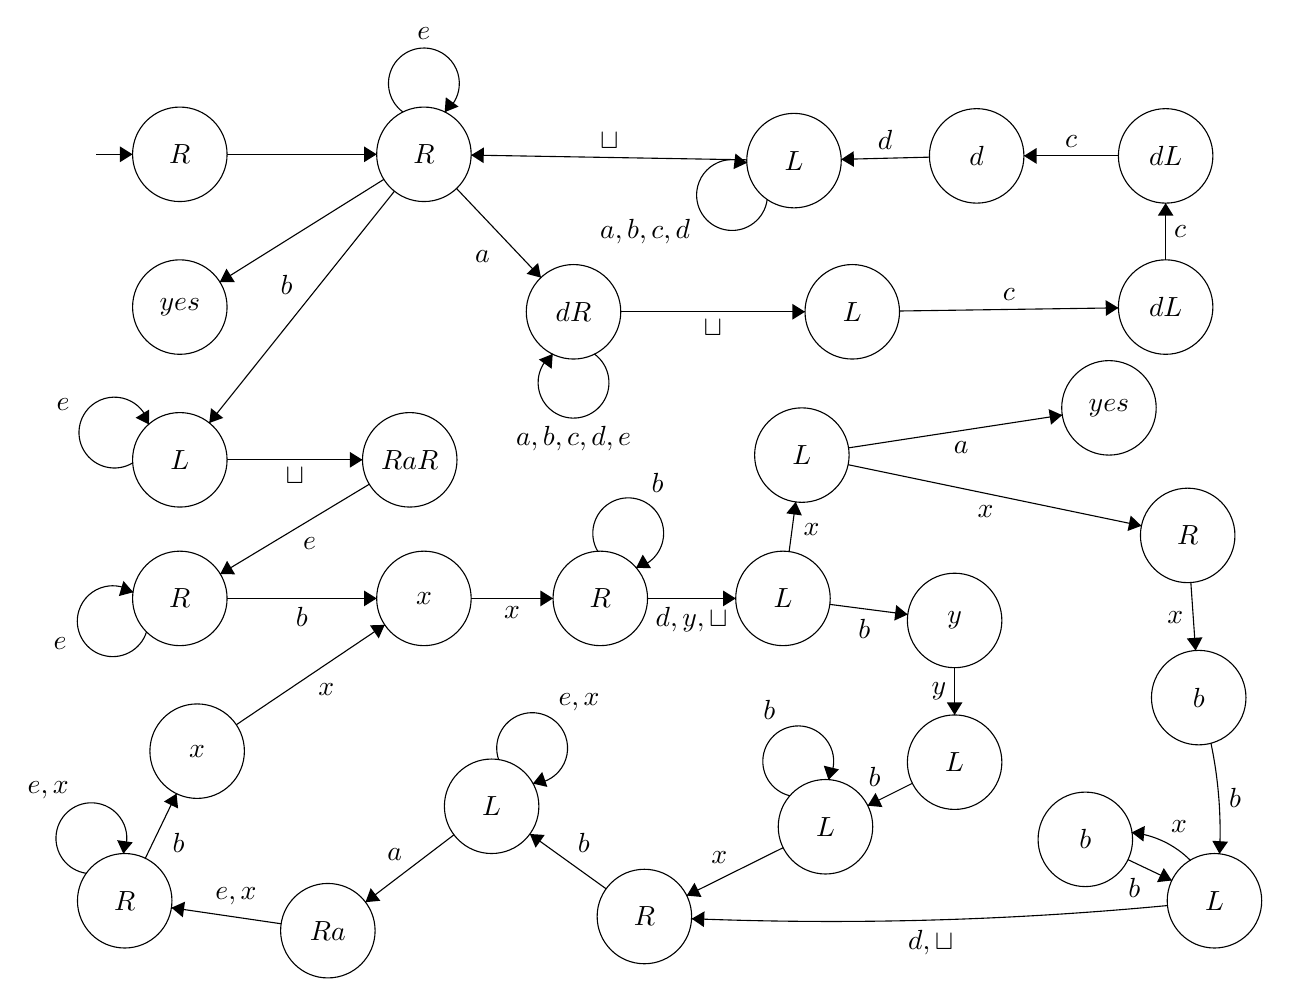
\begin{tikzpicture}[scale=0.2]
\tikzstyle{every node}+=[inner sep=0pt]
\draw [black] (10.1,-6.4) circle (3);
\draw (10.1,-6.4) node {$R$};
\draw [black] (25.6,-6.4) circle (3);
\draw (25.6,-6.4) node {$R$};
\draw [black] (10.1,-16.1) circle (3);
\draw (10.1,-16.1) node {$yes$};
\draw [black] (49.1,-6.8) circle (3);
\draw (49.1,-6.8) node {$L$};
\draw [black] (60.7,-6.5) circle (3);
\draw (60.7,-6.5) node {$d$};
\draw [black] (72.7,-6.5) circle (3);
\draw (72.7,-6.5) node {$dL$};
\draw [black] (72.7,-16.1) circle (3);
\draw (72.7,-16.1) node {$dL$};
\draw [black] (52.8,-16.4) circle (3);
\draw (52.8,-16.4) node {$L$};
\draw [black] (35.1,-16.4) circle (3);
\draw (35.1,-16.4) node {$dR$};
\draw [black] (10.1,-25.8) circle (3);
\draw (10.1,-25.8) node {$L$};
\draw [black] (10.1,-34.6) circle (3);
\draw (10.1,-34.6) node {$R$};
\draw [black] (24.7,-25.8) circle (3);
\draw (24.7,-25.8) node {$RaR$};
\draw [black] (25.6,-34.6) circle (3);
\draw (25.6,-34.6) node {$x$};
\draw [black] (36.8,-34.6) circle (3);
\draw (36.8,-34.6) node {$R$};
\draw [black] (48.4,-34.6) circle (3);
\draw (48.4,-34.6) node {$L$};
\draw [black] (49.6,-25.5) circle (3);
\draw (49.6,-25.5) node {$L$};
\draw [black] (69.1,-22.5) circle (3);
\draw (69.1,-22.5) node {$yes$};
\draw [black] (74.1,-30.6) circle (3);
\draw (74.1,-30.6) node {$R$};
\draw [black] (59.3,-36) circle (3);
\draw (59.3,-36) node {$y$};
\draw [black] (59.3,-45) circle (3);
\draw (59.3,-45) node {$L$};
\draw [black] (74.8,-40.9) circle (3);
\draw (74.8,-40.9) node {$b$};
\draw [black] (75.8,-53.8) circle (3);
\draw (75.8,-53.8) node {$L$};
\draw [black] (67.6,-49.9) circle (3);
\draw (67.6,-49.9) node {$b$};
\draw [black] (51.1,-49.1) circle (3);
\draw (51.1,-49.1) node {$L$};
\draw [black] (39.6,-54.8) circle (3);
\draw (39.6,-54.8) node {$R$};
\draw [black] (29.9,-47.8) circle (3);
\draw (29.9,-47.8) node {$L$};
\draw [black] (19.5,-55.7) circle (3);
\draw (19.5,-55.7) node {$Ra$};
\draw [black] (6.6,-53.8) circle (3);
\draw (6.6,-53.8) node {$R$};
\draw [black] (11.2,-44.3) circle (3);
\draw (11.2,-44.3) node {$x$};
\draw [black] (4.8,-6.4) -- (7.1,-6.4);
\fill [black] (7.1,-6.4) -- (6.3,-5.9) -- (6.3,-6.9);
\draw [black] (13.1,-6.4) -- (22.6,-6.4);
\fill [black] (22.6,-6.4) -- (21.8,-5.9) -- (21.8,-6.9);
\draw [black] (24.277,-3.72) arc (234:-54:2.25);
\draw (25.6,0.85) node [above] {$e$};
\fill [black] (26.92,-3.72) -- (27.8,-3.37) -- (26.99,-2.78);
\draw [black] (23.06,-7.99) -- (12.64,-14.51);
\fill [black] (12.64,-14.51) -- (13.59,-14.51) -- (13.06,-13.66);
\draw [black] (46.1,-6.75) -- (28.6,-6.45);
\fill [black] (28.6,-6.45) -- (29.39,-6.96) -- (29.41,-5.96);
\draw (37.37,-6.05) node [above] {$\sqcup$};
\draw [black] (27.67,-8.57) -- (33.03,-14.23);
\fill [black] (33.03,-14.23) -- (32.85,-13.3) -- (32.12,-13.99);
\draw (29.82,-12.87) node [left] {$a$};
\draw [black] (36.423,-19.08) arc (54:-234:2.25);
\draw (35.1,-23.65) node [below] {$a,b,c,d,e$};
\fill [black] (33.78,-19.08) -- (32.9,-19.43) -- (33.71,-20.02);
\draw [black] (38.1,-16.4) -- (49.8,-16.4);
\fill [black] (49.8,-16.4) -- (49,-15.9) -- (49,-16.9);
\draw (43.95,-16.9) node [below] {$\sqcup$};
\draw [black] (55.8,-16.35) -- (69.7,-16.15);
\fill [black] (69.7,-16.15) -- (68.89,-15.66) -- (68.91,-16.66);
\draw (62.75,-15.74) node [above] {$c$};
\draw [black] (72.7,-13.1) -- (72.7,-9.5);
\fill [black] (72.7,-9.5) -- (72.2,-10.3) -- (73.2,-10.3);
\draw (73.2,-11.3) node [right] {$c$};
\draw [black] (69.7,-6.5) -- (63.7,-6.5);
\fill [black] (63.7,-6.5) -- (64.5,-7) -- (64.5,-6);
\draw (66.7,-6) node [above] {$c$};
\draw [black] (57.7,-6.58) -- (52.1,-6.72);
\fill [black] (52.1,-6.72) -- (52.91,-7.2) -- (52.89,-6.2);
\draw (54.89,-6.12) node [above] {$d$};
\draw [black] (47.399,-9.257) arc (-6.95749:-294.95749:2.25);
\draw (42.53,-11.28) node [left] {$a,b,c,d$};
\fill [black] (46.12,-6.94) -- (45.38,-6.35) -- (45.26,-7.34);
\draw [black] (23.73,-8.74) -- (11.97,-23.46);
\fill [black] (11.97,-23.46) -- (12.86,-23.14) -- (12.08,-22.52);
\draw (17.29,-14.68) node [left] {$b$};
\draw [black] (7.118,-25.99) arc (301.38014:13.38014:2.25);
\draw (3.13,-22.28) node [left] {$e$};
\fill [black] (8.14,-23.55) -- (8.15,-22.61) -- (7.29,-23.13);
\draw [black] (13.1,-25.8) -- (21.7,-25.8);
\fill [black] (21.7,-25.8) -- (20.9,-25.3) -- (20.9,-26.3);
\draw (17.4,-26.3) node [below] {$\sqcup$};
\draw [black] (22.13,-27.35) -- (12.67,-33.05);
\fill [black] (12.67,-33.05) -- (13.61,-33.07) -- (13.1,-32.21);
\draw (18.34,-30.7) node [below] {$e$};
\draw [black] (7.988,-36.714) arc (-17.2522:-305.2522:2.25);
\draw (2.94,-37.49) node [left] {$e$};
\fill [black] (7.14,-34.21) -- (6.52,-33.49) -- (6.23,-34.45);
\draw [black] (13.1,-34.6) -- (22.6,-34.6);
\fill [black] (22.6,-34.6) -- (21.8,-34.1) -- (21.8,-35.1);
\draw (17.85,-35.1) node [below] {$b$};
\draw [black] (28.6,-34.6) -- (33.8,-34.6);
\fill [black] (33.8,-34.6) -- (33,-34.1) -- (33,-35.1);
\draw (31.2,-35.1) node [below] {$x$};
\draw [black] (36.641,-31.616) arc (210.77477:-77.22523:2.25);
\draw (40.43,-27.88) node [above] {$b$};
\fill [black] (39.07,-32.66) -- (40.02,-32.68) -- (39.5,-31.82);
\draw [black] (39.8,-34.6) -- (45.4,-34.6);
\fill [black] (45.4,-34.6) -- (44.6,-34.1) -- (44.6,-35.1);
\draw (42.6,-35.1) node [below] {$d,y,\sqcup$};
\draw [black] (52.57,-25.04) -- (66.13,-22.96);
\fill [black] (66.13,-22.96) -- (65.27,-22.58) -- (65.42,-23.57);
\draw (59.72,-24.59) node [below] {$a$};
\draw [black] (52.54,-26.11) -- (71.16,-29.99);
\fill [black] (71.16,-29.99) -- (70.48,-29.34) -- (70.28,-30.32);
\draw (61.26,-28.64) node [below] {$x$};
\draw [black] (48.79,-31.63) -- (49.21,-28.47);
\fill [black] (49.21,-28.47) -- (48.61,-29.2) -- (49.6,-29.33);
\draw (49.68,-30.2) node [right] {$x$};
\draw [black] (51.38,-34.98) -- (56.32,-35.62);
\fill [black] (56.32,-35.62) -- (55.59,-35.02) -- (55.47,-36.01);
\draw (53.56,-35.89) node [below] {$b$};
\draw [black] (74.3,-33.59) -- (74.6,-37.91);
\fill [black] (74.6,-37.91) -- (75.04,-37.07) -- (74.04,-37.14);
\draw (73.85,-35.79) node [left] {$x$};
\draw [black] (75.577,-43.796) arc (11.86795:-3.00261:27.216);
\fill [black] (76.12,-50.82) -- (76.66,-50.05) -- (75.66,-49.99);
\draw (76.69,-47.24) node [right] {$b$};
\draw [black] (70.538,-49.465) arc (84.37657:44.751:6.118);
\fill [black] (70.54,-49.46) -- (71.29,-50.04) -- (71.38,-49.05);
\draw (73.55,-49.52) node [above] {$x$};
\draw [black] (70.31,-51.19) -- (73.09,-52.51);
\fill [black] (73.09,-52.51) -- (72.58,-51.72) -- (72.15,-52.62);
\draw (70.71,-52.36) node [below] {$b$};
\draw [black] (59.3,-39) -- (59.3,-42);
\fill [black] (59.3,-42) -- (59.8,-41.2) -- (58.8,-41.2);
\draw (58.8,-40.5) node [left] {$y$};
\draw [black] (56.62,-46.34) -- (53.78,-47.76);
\fill [black] (53.78,-47.76) -- (54.72,-47.85) -- (54.28,-46.95);
\draw (54.21,-46.55) node [above] {$b$};
\draw [black] (48.849,-47.135) arc (256.61315:-31.38685:2.25);
\draw (47.54,-42.35) node [above] {$b$};
\fill [black] (51.29,-46.12) -- (51.96,-45.46) -- (50.99,-45.22);
\draw [black] (48.41,-50.43) -- (42.29,-53.47);
\fill [black] (42.29,-53.47) -- (43.23,-53.56) -- (42.78,-52.66);
\draw (44.36,-51.45) node [above] {$x$};
\draw [black] (72.815,-54.104) arc (-84.56759:-92.2677:225.109);
\fill [black] (42.6,-54.94) -- (43.38,-55.47) -- (43.42,-54.47);
\draw (57.78,-55.63) node [below] {$d,\sqcup$};
\draw [black] (37.17,-53.04) -- (32.33,-49.56);
\fill [black] (32.33,-49.56) -- (32.69,-50.43) -- (33.27,-49.62);
\draw (35.75,-50.8) node [above] {$b$};
\draw [black] (30.347,-44.845) arc (199.13726:-88.86274:2.25);
\draw (35.45,-41.76) node [above] {$e,x$};
\fill [black] (32.52,-46.36) -- (33.44,-46.57) -- (33.11,-45.62);
\draw [black] (27.51,-49.61) -- (21.89,-53.89);
\fill [black] (21.89,-53.89) -- (22.83,-53.8) -- (22.22,-53);
\draw (23.75,-51.25) node [above] {$a$};
\draw [black] (16.53,-55.26) -- (9.57,-54.24);
\fill [black] (9.57,-54.24) -- (10.29,-54.85) -- (10.43,-53.86);
\draw (13.66,-54.09) node [above] {$e,x$};
\draw [black] (7.91,-51.1) -- (9.89,-47);
\fill [black] (9.89,-47) -- (9.09,-47.5) -- (9.99,-47.94);
\draw (9.61,-50.13) node [right] {$b$};
\draw [black] (4.173,-52.057) arc (262.04213:-25.95787:2.25);
\draw (1.74,-47.34) node [above] {$e,x$};
\fill [black] (6.51,-50.81) -- (7.11,-50.09) -- (6.12,-49.95);
\draw [black] (13.69,-42.62) -- (23.11,-36.28);
\fill [black] (23.11,-36.28) -- (22.17,-36.31) -- (22.73,-37.14);
\draw (19.4,-39.95) node [below] {$x$};
\end{tikzpicture}
\end{center}

\subsection*{b.}
The grammer is as follows:\\
\begin{itemize}
	\item $S_1 \rightarrow$ b | S
	\item S $\rightarrow$ aBccc | aBSccc
	\item Ba $\rightarrow$ aB
	\item aB $\rightarrow$ aB$\delta$
	\item P $\rightarrow$ e
	\item $delta$ $\rightarrow$ e
	\item PB $\rightarrow$ P
	\item bB $\rightarrow$ Bbb
	\item b$\delta$B $\rightarrow$ bB$\delta$
	\item B$\delta$ $\rightarrow$ PbB$\delta$
\end{itemize}



\section*{Answer 6}

\subsection*{a.}
\textbf{$L_1$}\\
Since regular grammers are subset of the context free grammers, they are context free and recursively enumerable. We can conclude that there exists a turing machine $M_1$ that recognizes regular grammers.\\
\textbf{$L_2$}\\
If we generalize the context free grammers, we get the unrestricted grammers and to generate a language by using grammer, it must be recursively enumerable. Furthermore, recursively enumerable languages are accepted by the Turing machines, there exits a turing machine $M_2$ which accepts the language $L_2$.\\
\textbf{$L_3$}\\
Same logic with $L_2$ and $M_2$.\\
\textbf{$L_4$}\\
The second part of the given language which is $bar{a^*b^*}$ is regular, since it complementation of a regular language and regular languages are closed under complementation. Moreover, the $\bar{L_4}\cap\bar{a^*b^*}$ is recursively enumerable since a turing machine accepts it. $L_4$ must be a recursively enumerable, to that language be recursively enumerable. Since $L_4$ is recursively enumerable, there exits a turing machine $M_4$ which accepts the language $L_4$.\\
\textbf{$L_5$}\\
Same logic with $L_2$ and $L_3$.\\
\subsection*{b.}
Sinec $L_1,L_2,L_3$ are context free or regular language, they have algorithms. Regular languages are recursive, since it has finitely many states and has no memory, thus, we can say that finite automaton will always stop. Context free languages are recursive since the push down automaton that recognizes context free languages has finite input and stack, and that will also always stop.
However, $L_4$ and $L_5$ cannot have algorithm for some cases, since they are recursively enumerable languages, and recursively enumerable languages are the superset of the recursive languages.\\

\subsection*{c.}
We should define two machines one recognizes $\bar{L_2}L_1 \cap L_5$ and the other recognizes $L_3^*\bar{L_4}$. \\
To recognize $L_3^*\bar{L_4}$, the machine $M_Y$:\\
In accepting states of $M_3$ is going either starting state of the $M_4$ or starting states of itself.
To recognize $\bar{L_2}L_1 \cap L_5$, the machine $M_X$:\\
It should copy the given string as sxs where x not in $\Sigma$. After that, it should move through to first string s and determine whether it is in the language $\bar{L_2}L_1$. After that, it moves through the second string s and determine whether it is in the language $L_5$. If both conditions are satisfied, it should accept the string.\\
We should have a machine that include both of the machine we defined. It should choose undeterministicly $M_X$ and $M_Y$. If one the machines accept the string, then the string is accepted.

\subsection*{d.}

%Do not submit solutions for Question 7, yet do solve it.


\end{document}

​

